This problem is very interesting and I consider that is better to make an analysis using some draws, imagine that you want to generate binary numbers from 1 to 5, if we do this first we need to add a '1' to our queue (our queue needs to be of strings) then we have two options add a '1' to this string or '0' it generates a new binary string, for example: Let's imagine that we want generate binary strings from 1 to 7, we have a procees like the next:

\begin{figure}[H]
    \centering
    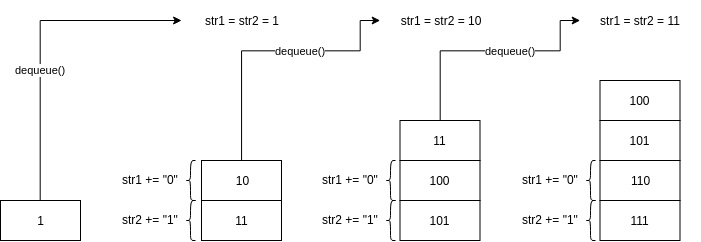
\includegraphics[width=1.00\textwidth]{Images/DataStructures/Queue/queue_example.png}
    \caption{Problem 03 diagram}
    \label{fig:queue-problem-03}
\end{figure}

As you can see we only need to to enqueue a new string using the top of our queue and concatenating an extra character first a zero and then a one, and we made the same as many times as we need. If we code this we have the next as a result:

\begin{lstlisting}
    #include <bits/stdc++.h>

    using namespace std;

    int main(){
        
        queue<string> Queue;
        string str1, str2;
        int n;
        cin >> n;
        Queue.push("1");
        for(int i = 0; i < n; i++){
            str1 = Queue.front();
            str2 = Queue.front();
            Queue.pop();
            cout << str1 << endl;
            str1 += "0";
            str2 += "1";
            Queue.push(str1);
            Queue.push(str2);
        }
        return 0;
    }
\end{lstlisting}